\documentclass[a4paper,12pt]{report}
\usepackage{color}
\usepackage{graphicx}
\usepackage{subfig}
\usepackage{listings}
\usepackage{movie15}
\usepackage{hyperref}

\definecolor{dkgreen}{rgb}{0,0.6,0}
\definecolor{gray}{rgb}{0.5,0.5,0.5}
\definecolor{mauve}{rgb}{0.58,0,0.82}

\begin{document}

\title{CSC190 Notes}
\author{Aman Bhargva}
\date{January-April 2019}
\maketitle

\tableofcontents

\section{Introduction and Course Information}

\chapter{Efficiency and Complexity}
There are two things that effect efficiency of a computer algorithm.
\begin{itemize}
\item Space Complexity = cost in terms of memory
\item Time Complexity = cost in terms of steps
\end{itemize}

\section{Ideal vs. Real Computers}
\begin{tabular}{l|l}
Ideal & Real \\
\hline
Automaton + Workbook & Microprocessor + Memory \\
Mathematical Algorithms & Programs (Sea of Functions) \\
Abstract Data Types & Data Structure 
\end{tabular}

\texttt{Note: ADTs are Abstract Data Types}

Stack is used by C for temporary variables made by functions. Heap is used by CPU and by malloc. All stuff pushed to the stack by a function is freed when the function exits. 

\section{The RAM Model of Computation}
Stands for Random Access Machine Model.
Each simple operation takes 1 time step. Each memory access takes 1 time step. It's actually a really good models for how computers perform.

\subsection{Big Oh Notation}
Usually used for worst case scenarios.
\begin{itemize}
\item $O(g(n))$ is for upper bound of time complexity.
\item $\Omega(g(n))$ is for lower bound of time complexity.
\item $\Theta(g(n))$ is for upper AND lower bound (separated by only a constant)
\end{itemize}

\subsubsection{Dominance Classes}
One class of algorithms in big Oh notation is said to dominate another if their time complexity grows faster than the other.
\begin{enumerate}
\item Linear
\item Logarithmic
\item Linear
\item Super Linear ($n log(n)$)
\item Quadratic
\item Cubic
\item Exponential
\item Factorial
\end{enumerate}
	

\chapter{List ADT implementation in C}
\begin{itemize}
\item An array with length L and end index 'end'
\end{itemize}

\section{Stacks and Queues}
\subsection{Stacks}
\begin{itemize}
\item First in, last out
\item push and pop
\end{itemize}
\subsection{Queues}
\begin{itemize}
\item First in, first out
\item enqueue, dequeue
\end{itemize}

\chapter{Trees}
\section{Types of General Traversal:}
\subsubsection{Breadth-First Traversal: }
In which you read (1) right to left (2) top to bottom.
\subsubsection{Depth-First Traversal: }
In which you read (1) top to bottom (2) right to left

\subsection{Using Stacks and Queues for Traversals}
\paragraph{Remember: } Stacks $\to$ Depth-First. Queues $\to$ Breadth-First. 
\paragraph{How does it work?}
On inspection, you would think that recursion is the only way to effectively traverse a tree in a depth/breadth-first manner in an easy way. However, you can employ stacks and queues to do this iteritavely. Here are the steps:
\begin{enumerate}
\item Add the root node to the {stack, queue} per the above statement.
\item Pop/dequeue the dequeueing point and print it. Add its children to the {stack, queue}
\item Repeat step 2 until finished. 
\end{enumerate}
This isn't immediately intuitive, but it holds true. Try this on a tree on paper to convince yourself! It's a really cool property of trees/stacks/queues :)

\section{Binary Trees: }
\subsection{Mathai's Weird Definition for Binary Trees vs. Normal Trees}
The rule: The first child of a node goes as the left child in the binary tree. All of its siblings are added as RIGHT children of that first child. Etc.
\subsection{Binary Search Trees: }
Think about the binary search algorithm. The rule is simple: Start with the first node. If the thing you want to add is greater than that node, you add it to the RIGHT child tree. Otherwise, you add it to the LEFT child tree. The rule is recursive and super elegant.
\subsection{Advantages/Disadvantages of Binary Search Trees: }
\begin{enumerate}
\item Advantage: Will (generally) change search from O(n) to O(log(n)) because you only need to visit every LEVEL instead of every NODE (\#levels = log(\#nodes))
\item Disadvantage: If it's not a balanced tree, you could end up with a BST that has \#levels = \#nodes
\end{enumerate}

\subsection{Binary Tree Traversals}
\begin{enumerate}
\item Pre-Order: NLR
\item Post-Order: LRN
\item In-Order: LNR
\end{enumerate}
\paragraph{Mnemonic: } The 'pre'/'post'/'in' refers to the placement of the NODE between/in front of/after the L and R node.

\section{Self-Balancing BST's (AVL Trees): }
The general way we balance binary search trees is with \textbf{rotations}
\paragraph{Level of imbalance: } calculated as nR (number of levels on the right side of the node) minus nL.
\paragraph{Printing Binary Trees in Order: } When you print the left subtree first, then the node, then the right subtree (recursively)
\subsubsection{Types of Rotation: }
\begin{enumerate}
\item Left
\item Right
\item Major Left / Minor Right
\item Major Right / Minor Left
\end{enumerate}

\subsection{Right Rotation: }
The left child becomes the head. The left child's parent (the root) becomes the right child, and the left child of the left child becomes maintains its relationship with the left child of the root. The original left child's RIGHT child becomes the left child of the original root. 
\paragraph{When to do this? } whenever nL - nR $\geq$ 2...?

\subsection{Left Rotation: }
The right child becomes the head. The right child's parent (the root) becomes the left child, and the right vhild of the right child maintains its relationship with the right child of the original root. The original right child's LEFT child becomes the right child of the original root. 

\subsection{Major Right / Minor Left: }
\paragraph{When to do this: } Whenever the balance on the root and the balance on a subtree is opposite, and the absolute balance of the root is greater than or equal to 2. Tl;dr: You want the subtrees to have the same SIGN of balance as the root node before you do big switches. Condition for doing compelex switches is: balance (root) >=2, sign balance (sub-node) doesn't equal the sign balance (root node)

\subsection{Summary of Tree Rotations: }
\begin{enumerate}
\item For easy, child-free lines to the right and left (root balance = +-2, child banace = +-1 with same sign), use the corresponding rotation to make them triangle trees.
\item For bent ones with root balance = +-2 and child balance +-1 of opposite sign), use minor rotation to get back to case 1 and do a major rotation on the root. 
\end{enumerate}

\begin{figure}[h]
\centering
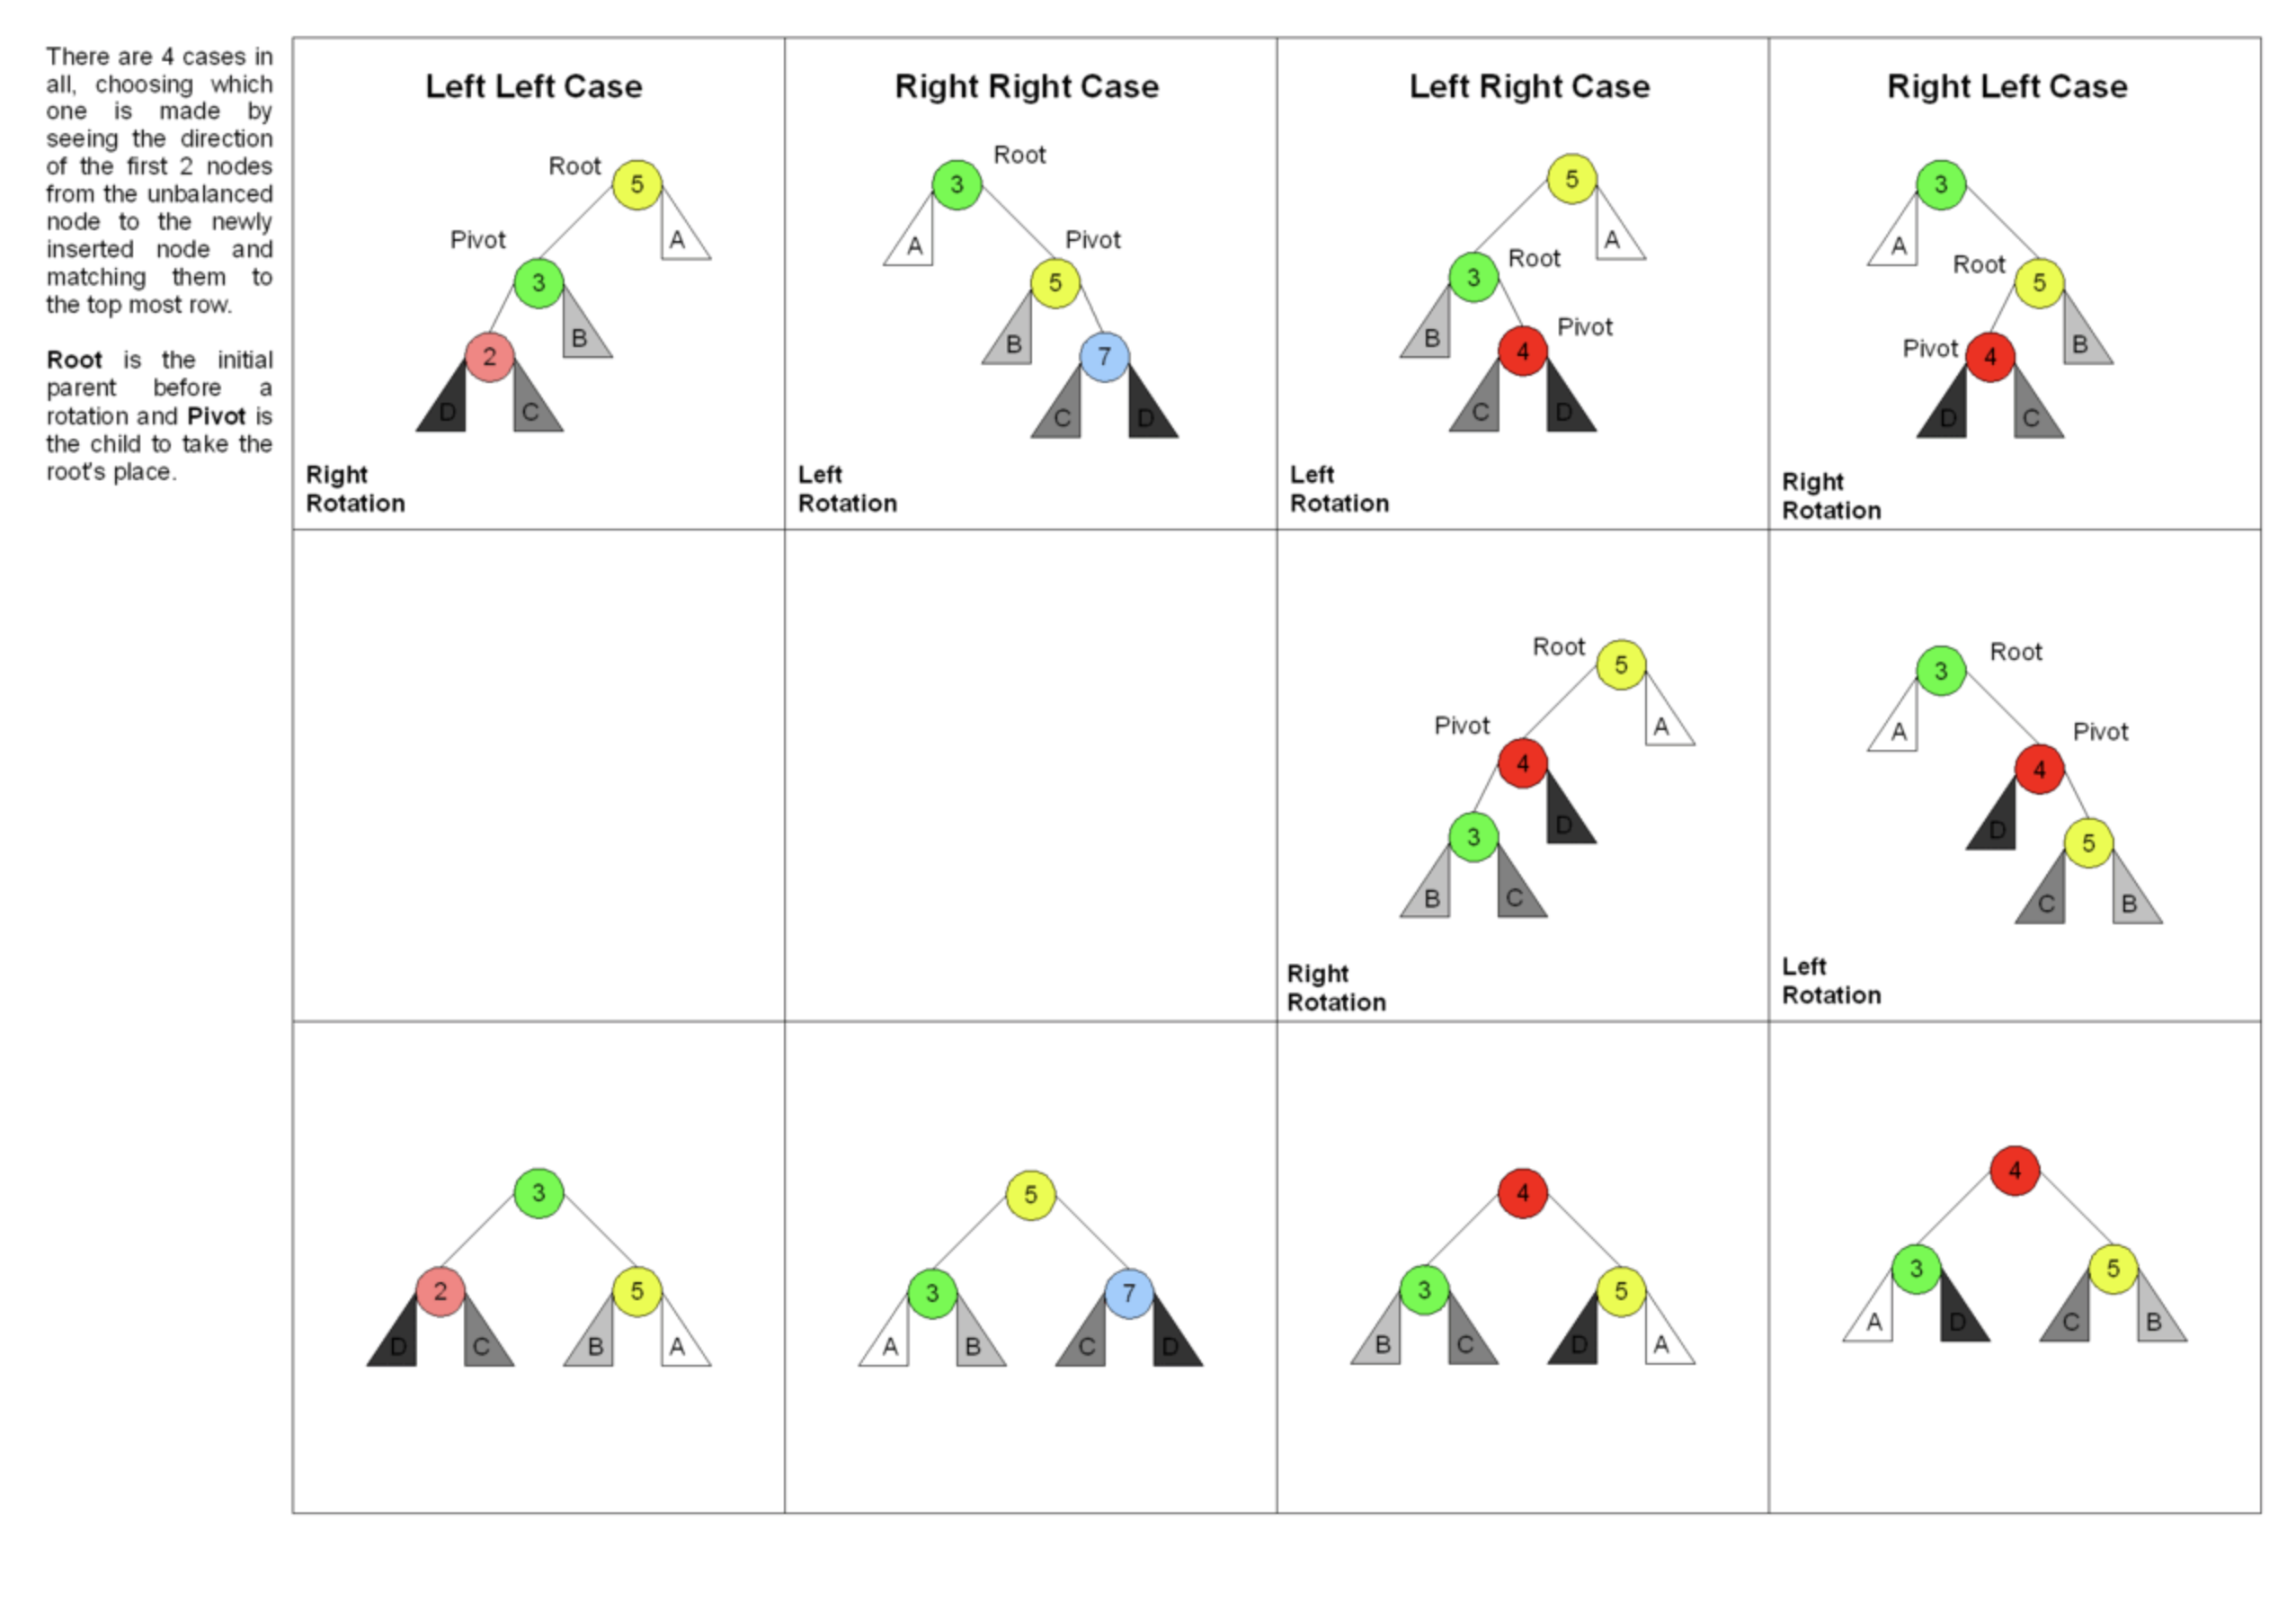
\includegraphics[width=1\textwidth]{media/tree-rotation-summary.png}
\caption{Summary of All Rotation Types}
\label{Tree Rotation Summary}
\end{figure}


\begin{figure}%
    \centering
    \subfloat[label 1]{{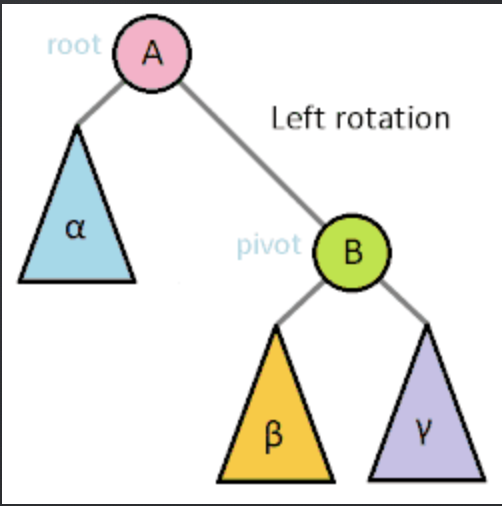
\includegraphics[width=5cm]{media/left-rotation-1.png} }}%
    \qquad
    \subfloat[label 2]{{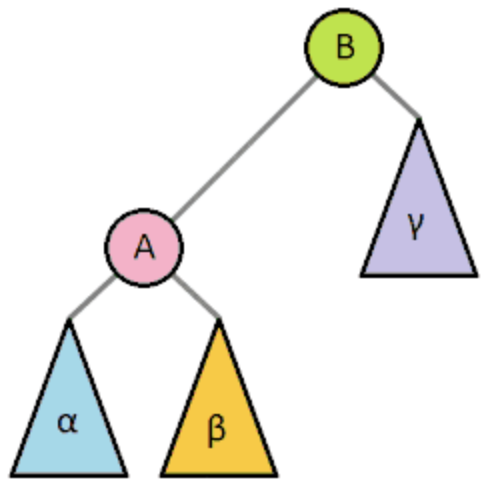
\includegraphics[width=5cm]{media/left-rotation-2.png} }}%
    \caption{Visual Representation of a Left Rotation}%
    \label{fig:example}%
\end{figure}


\begin{figure}%
    \centering
    \subfloat[label 1]{{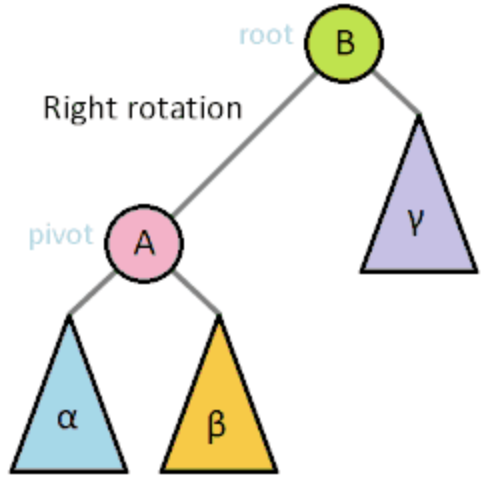
\includegraphics[width=5cm]{media/right-rotation-1.png} }}%
    \qquad
    \subfloat[label 2]{{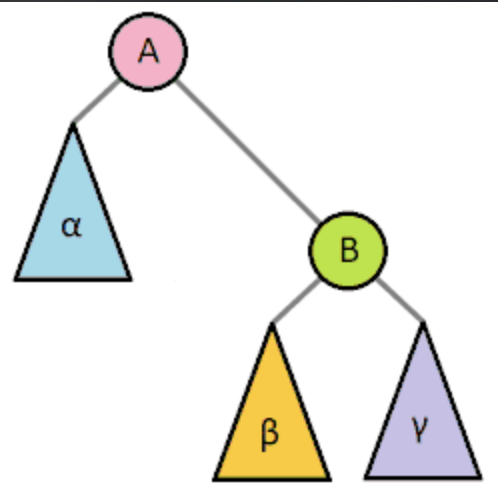
\includegraphics[width=5cm]{media/right-rotation-2.png} }}%
    \caption{Visual Representation of a Right Rotation}%
    \label{fig:example}%
\end{figure}

\subsection{Inserting to a Binary Tree}
\begin{enumerate}
\item If we are passed a pointer to a NULL pointer, then add this info as the NULL pointer.
\item If we are passed a node:
\item Add to the left subtree if we are smaller than that particular node.
\item Add to the right subtree otherwise.
\end{enumerate}


\subsection{Deleting from a Binary Tree}
Swap the node you need to delete with the left child's furthest right child. Then delete the initial node. Also works with the right child's firthest left descendant. Think about how repeated elements might change this up. 

\section{AVL Tree}
AVL trees are self-balancing BST's.
\subsection{When to use which rotation/HOW TO BALANCE: }
Lines of two and zigzags of two are the worst case scenario and they're all you'll ever really have to deal with.
Always do rotations on things that have +/- 2. 

\subsection{Adding to AVL Trees: }
Do binary insert. Then balance it. 

\subsection{Deleting from AVL Trees: }
Do binary deletion. Then balance it.

\section{Priority Queues}
Operations:
\begin{enumerate}
\item Insert element
\item Find minimum
\item Find maximum
\end{enumerate}

The queue can be an ordered list, unordered list, binary search tree, and more. 

\section{Hashes and Strings}
Hashes = way to maintain a dictionary. Takes advantage of $O(n)$ complexity of finding something once you know its key (location) in a list/array. 

\paragraph{Example: } indexing strings. Hash function uses each letter as a number in a base-alphabet number system. Then you map any string to unimaginably large numbers. To find where they should go in an array, take the output \% the size of the array.

\paragraph{Problem: } you're likely to have some collisions in terms of where you assigned a string. Let $m$ be the length of the array. 

\paragraph{Solution 1: Chaining } where you have linked lists for each hash table entry that has multiple items hashing to it. But this uses a lot of memory for pointers.

\paragraph{Solution 2: Open Addressiong } where you just chuck it in the next sequentially available slot. It's not great though because repeated deletion and addition may result in an entirely random hash table.  

\section{Heap}
Max heap = top heavy. Min heap = bottom heavy.
\subsection{Implementation as List}
\begin{enumerate}
\item Child Index = Parent Index...
\item ...
\end{enumerate}

\subsection{Adding to a Heap}
\begin{enumerate}
\item Add to the last element in the heap/list
\item If parent and child relationship is OK, then stop.
\item Otherwise, swap and go back to step 2.
\end{enumerate}

\subsection{Deleting from Heap}
\begin{enumerate}
\item Replace deleted item with the item furthest down and to the right in the heap.
\item Heapify by swapping with parent if necessary or with child if necessary.
\end{enumerate}

\subsection{Searching a Heap}
You have to search everything. But you can stop if you reach something larger (in the case of a min heap) or smaller (in the case of a max heap). 


\end{document}
